\documentclass[12pt]{ociamthesis}  % default square logo 
%\documentclass[12pt,beltcrest]{ociamthesis} % use old belt crest logo
%\documentclass[12pt,shieldcrest]{ociamthesis} % use older shield crest logo

%load any additional packages
\usepackage{amssymb}
\usepackage{listings}
\usepackage{float}
\usepackage{graphics}
\usepackage{color}
 
\definecolor{codegreen}{rgb}{0,0.6,0}
\definecolor{codegray}{rgb}{0.5,0.5,0.5}
\definecolor{codepurple}{rgb}{0.58,0,0.82}
\definecolor{backcolour}{rgb}{0.95,0.95,0.92}
 
\lstdefinestyle{mystyle}{
    backgroundcolor=\color{backcolour},   
    commentstyle=\color{codegreen},
    keywordstyle=\color{magenta},
    numberstyle=\tiny\color{codegray},
    stringstyle=\color{codepurple},
    basicstyle=\footnotesize,
    breakatwhitespace=false,         
    breaklines=true,                 
    captionpos=b,                    
    keepspaces=true,                 
    numbers=left,                    
    numbersep=5pt,                  
    showspaces=false,                
    showstringspaces=false,
    showtabs=false,                  
    tabsize=2,
    language=python
}
 
\lstset{style=mystyle}

%input macros (i.e. write your own macros file called mymacros.tex 
%and uncomment the next line)
%\include{mymacros}

\title{Tugas Chapter 4\\[1ex]     %your thesis title,
        Pemrograman II}   %note \\[1ex] is a line break in the title

\author{Yusuf Jordan El Anwar}             %your name
\college{1184026\\[5ex]
Applied Bachelor of Informatics Engineering}  %your college

%\renewcommand{\submittedtext}{change the default text here if needed}
\degree{Politeknik Pos Indonesia}     %the degree
\degreedate{Bandung 2019}         %the degree date

%end the preamble and start the document
\begin{document}

%this baselineskip gives sufficient line spacing for an examiner to easily
%markup the thesis with comments
\baselineskip=18pt plus1pt

%set the number of sectioning levels that get number and appear in the contents
\setcounter{secnumdepth}{3}
\setcounter{tocdepth}{3}


\maketitle                  % create a title page from the preamble info
\begin{dedication}
`Jika Kamu tidak dapat menahan lelahnya belajar, \\
Maka kamu harus sanggup menahan perihnya Kebodohan.'\\ 
~Imam Syafi'i~\\
\end{dedication}        % include a dedication.tex file

\begin{romanpages}          % start roman page numbering
				
\end{romanpages}            % end roman page numbering



%now include the files of latex for each of the chapters etc
\chapter*{Teori}

\begin{enumerate}
	\item CSV(Comma Separated Value) adalah format data yang digunakan para pengguna untuk menginputkan data kedalam database secara sederhana.

	\begin{itemize}
	\item Fungsi file CSV adalah format basis data sederhana yang di setiap record dipisahkan dengan tanda koma dan titik koma.
	\end{itemize}
	
	\begin{figure} [h]
	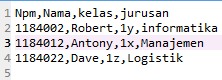
\includegraphics[width=5cm]{poto/1.png}
	\centering
	\end{figure}		
	
	
	
	
	\item Aplikasi yang dapat membuat file CSV adalah Notepad,Worpad,Microsoft Excel,dll
	
	\item Cara membuat file CSV:
	\begin{itemize}
	\item Buka Ms.Excell
	\end{itemize}
	\begin{itemize}
	\item Membuat data di Ms.Excel
	\end{itemize}
	\begin{itemize}
	\item Lalu pada saat menyimpan pilih "save as" dan jenis file nya diganti csv
	\end{itemize}
	\begin{itemize}
	\item Dan file CSV telah dibuat
	\end{itemize}

	\item library csv adalah format yang sudah digunakan selama bertahun-tahun dengan cara standar di RFC 4180. Perbedaan halus terdapat di beberapa aplikasi.
	
	
	\item library Pandas adalah alat analisis data dan struktur unruk bahasa pemrograman Python.  Panda digunakan dengan mudah untuk mengelola data salah satu fiturnya adalah Dataframe. Dataframe dapat digunakan untuk membaca sebuah file dan menjadikannya table.


	\item Fungsi yang terdapat pada library CSV:\\
	\begin{itemize}
	\item Reade, Fungsi Reader diguunakan untuk membaca  isi file
	\end{itemize}
	\begin{itemize}
	\item Dict Reader, Fungsi Dict Reader digunakan untuk membaca isi file yang terdapat di dictionary
	\end{itemize}
	\begin{itemize}
	\item Write, Fungsi Write ini digunakan untuk menulis file
	\end{itemize}
	\begin{itemize}
	\item Dict Write, Fungsi Dict Write digunakan untuk menulis file yang ada di dictionary
	\end{itemize}
	
	\item Fungsi yang terdapat di libarary pandas
	\begin{itemize}
	\item to\_csv, untuk menulis file yang type nya CSV
	\end{itemize}
	\begin{itemize}
	\item read\_csv, untuk membaca file type CSV
	\end{itemize}
	
	
\end{enumerate}



\chapter{Ketrampilan Pemrograman}

\section{Nomor 1}
\lstinputlisting[language=Python, firstline=4, lastline=8]{src/1184047_realtime.py}
\section{Nomor 2}
\lstinputlisting[language=Python, firstline=3, lastline=8]{src/1184047_save.py}
\section{Nomor 3}
\lstinputlisting[language=Python, firstline=10, lastline=18]{src/1184047_realtime.py}
\section{Nomor 4}
\lstinputlisting[language=Python, firstline=4, lastline=16]{src/1184047_csv.py}
\chapter{Laporan}
\section{PEMAHAMAN TEORI}
\subsection{FUNGSI}
\begin{enumerate}
	\item Fungsi adalah salah satu blok program yang sudah terorganisir terdiri dari nama fungsi, input variabel dan variabel kembalian. Fungsi digunakan untuk aplikasi anda dan tingkat penggunaan kode yang tinggi agar aplikasi lebih baik.
	\item inputan fungsi digunakan untuk menerima baris input dari user dan mengembalikannya dalam bentuk string.
	\item kembalian fungsi yaitu fungsi akan membaca sebaris input umumnya melalui keyboard sampai nanti dijumpai karakter newline(enter) dan akan mengembalikan string dari inputan tersebut.  
\end{enumerate}
\lstinputlisting[language=Python]{src/KodingTeori1.py}

\subsection{PAKET}
\begin{enumerate}
\item Paket adalah sebuah manifestasi dari konsep namespace hierarkis python.
\item cara pemanggilan paket  
\lstinputlisting[language=Python]{src/KodingTeori2.py}
\end{enumerate}

\subsection{KELAS}
\begin{enumerate}
\item kelas adalah prototipe yang ditentukan oleh pengguna untuk objek yang mendefinisikan seperangkat atribut yang menjadi ciri khas dari sebuah kelas apa pun. Class digunakan untuk membuat kelas baru dan nama kelas diikuti kanca kunci titik dua. 
\item Objek adalah perwujudan dari sebuah class. Bila kelas adalah prototipe nya, dan objek adalah barang jadinya. 
\item atribut yaitu semua class yang membuat objek dan semua objek tersebut mengandung karakteristik.
\item method merupakan fungsi yang didefinisikan di dalam suatu class.
\end{enumerate}
\lstinputlisting[language=Python]{src/KodingTeori3.py}
\subsection{Cara pemanggilan library kelas dari instansiasi dan pemakaiannya contoh dengan program}
untuk membuat objek dari sebuah kelas, kita memanggil nama kelas dengan argumen yang sesuai dengan   fungs pada saat kita mendefinisikannya.
\\cara pemanggilan\\
\lstinputlisting[language=Python]{src/KodingTeori4.py}
\subsection{Pemakaian paket dengan perintah from kalkulator import penambahan}
Pertama-tama kalian harus membuat program kalkulator.py untuk bisa melakukan penambahan sperti di bawah
\lstinputlisting[language=Python]{src/KodingTeori5.py}
\subsection{Pemakaian paket fungsi apabila file library ada di dalam folder}
Untuk pemakaian paket fungsi apabila file library berada di folder yaitu untuk dapat melakukan atau menjalankan kalkulator yang berada di file folder.
\lstinputlisting[language=Python]{src/KodingTeori6.py}
\subsection{Pemakaian paket kelas apabila file library ada di dalam folder}
Untuk pemakaian paket kelas apabila file library berada di folder.Mahasiswa yaitu file Mahasiswa untuk melakukan atau menjalankan kode yang berada di file folder Mahasiswa tersebut.
\lstinputlisting[language=Python]{src/KodingTeori7.py}
\section{KETERAMPILAN PEMROGAMAN}
\lstinputlisting[language=Python]{src/NPM1.py}
\lstinputlisting[language=Python]{src/NPM2.py}
\lstinputlisting[language=Python]{src/NPM3.py}
\lstinputlisting[language=Python]{src/NPM4.py}
\lstinputlisting[language=Python]{src/NPM5.py}
\lstinputlisting[language=Python]{src/NPM6.py}
\lstinputlisting[language=Python]{src/NPM7.py}
\lstinputlisting[language=Python]{src/NPM8.py}
\lstinputlisting[language=Python]{src/NPM9.py}
\lstinputlisting[language=Python]{src/NPM10.py}
\lstinputlisting[language=Python]{src/kalkulator.py}
\lstinputlisting[language=Python]{src/Mahasiswa.py}
\lstinputlisting[language=Python]{src/Ngitung.py}
\lstinputlisting[language=Python]{src/3lib.py}
\lstinputlisting[language=Python]{src/main.py}
\lstinputlisting[language=Python]{src/kelas3lib.py}
\lstinputlisting[language=Python]{src/main.py}
\section{KETERAMPILAN PENANGANAN ERROR}
\lstinputlisting[language=Python]{src/KeterampilanPenangananError.py}
\section{LAMPIRAN PLAGIARISM}
\begin{figure}[H]
		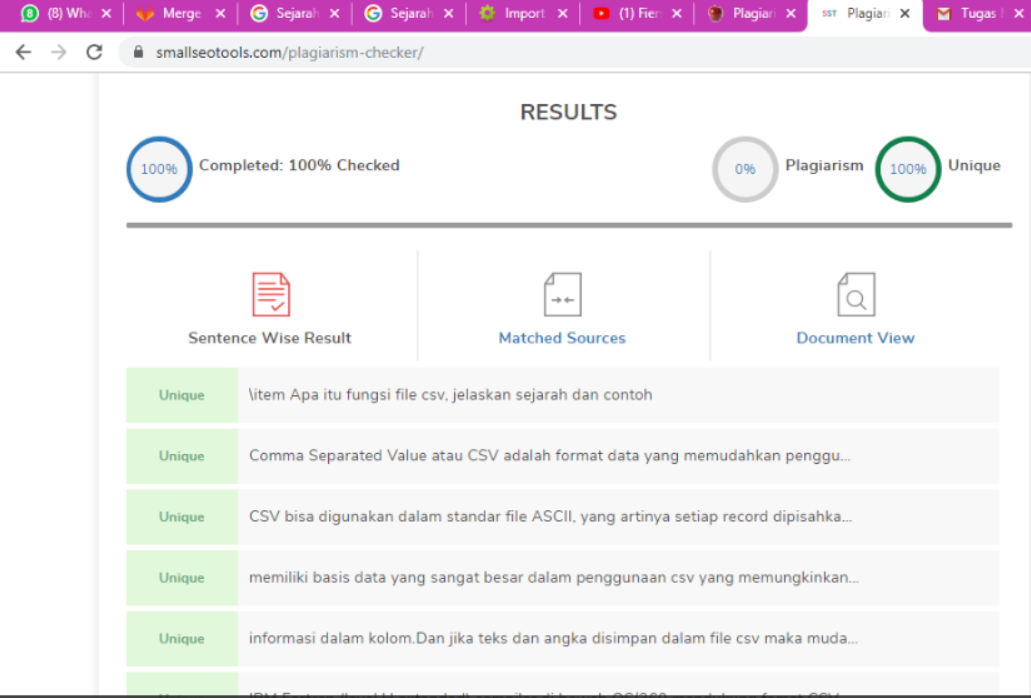
\includegraphics[width=4cm]{figures/1184065/ss1.PNG}
		\centering
		\caption{Screnshoot Plagiarism}
	\end{figure}
	\begin{figure}[H]
		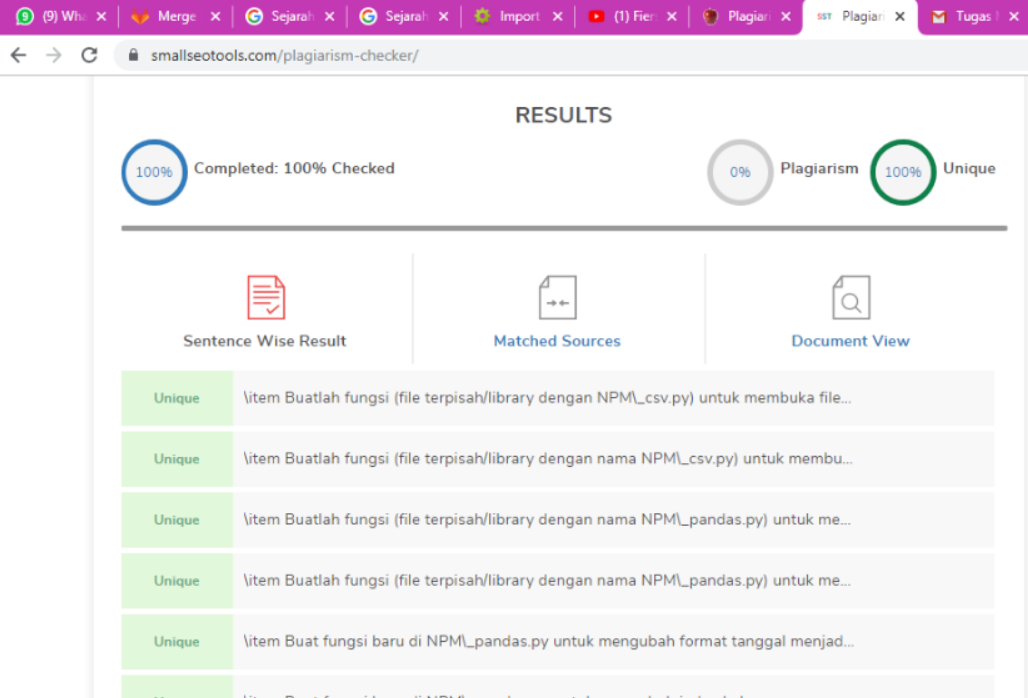
\includegraphics[width=4cm]{figures/1184065/ss2.PNG}
		\centering
		\caption{Screnshoot Plagiarism}
	\end{figure}
\section{LINK YOUTUBE}
\begin{enumerate}
\item \href{https://youtu.be/FDE8KrHC4m4}{klik}
\item \href{https://youtu.be/qzmEN1LVhsM}{klik}
\item \href{https://youtu.be/3UKVrJmwmYo}{klik}
\item \href{https://youtu.be/3UKVrJmwmYo}{klik}
\end{enumerate}









%now enable appendix numbering format and include any appendices
\appendix


%next line adds the Bibliography to the contents page

\end{document}

